\documentclass[border=2pt]{standalone}
\usepackage{tikz}
\usetikzlibrary{positioning,arrows.meta}
\begin{document}
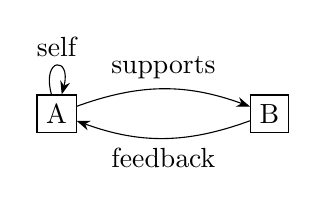
\begin{tikzpicture}
  \node[draw] (a) {A}; \node[draw,right=22mm of a] (b) {B};
  \draw[-{Stealth}] (a) to[bend left=20] node[above]{supports} (b);
  \draw[-{Stealth}] (b) to[bend left=20] node[below]{feedback} (a);
  \draw[-{Stealth}] (a) to[loop above] node[above]{self} (a);
\end{tikzpicture}
\end{document}
